%%% Laboratory	 Notes
%%% Template by Mikhail Klassen, April 2013
%%% Contributions from Sarah Mount, May 2014
%%% Contributions from Muhammad Davi, September 2022
\documentclass[a4paper]{tufte-handout}
\usepackage{lab_notes}

\title{Practice Big Data}
\date{2022}

\begin{document}
\maketitle

%%%%%%%%%%%%%%%%%%%%%%%%%%%%%%%%%%%%%%%%%%%%%%%%%%%%%%%%

\begin{projects}
\begin{description}
\item [Muhammad Davi, S.Kom., M.Cs.] adalah sebagai dosen pengampu matakuliah practice big data\footnote{Dosen Prodi Teknologi Rekayasa Komputer Jaringan, Jurusan Teknologi Informasi dan Komputer, Politeknik Negeri Lhokseumawe}.
\item [Peserta dan Kelompok] matakuliah practice big data adalah sebegai berikut:

\begin{table}[!ht]
\caption{Peserta dan Kelompok Matakuliah Practice Big Bata}
\label{tab:peserta}
\centering
\begin{tabular}{ll} 
\toprule
Nama &	Akun Github\\
\midrule
Kelompok 1\\
\midrule
FaziaFathin				  & \url{https://github.com/FaziaFathin} \\
Nadila Auliya	      & \url{https://github.com/NadilaAuliya} \\
Putri Zara Nisfu		& \url{https://github.com/putrizaranisfu} \\
\midrule
Kelompok 2\\
\midrule
Zatus Sakina				& \url{https://github.com/ZatusSakina} \\
Lukmanul Hakim			& \url{https://github.com/SayedLukmanulHakim} \\
Siti Nadifa			& \url{https://https://github.com/SitiNadifa} \\
Leuwi Alsraf		& \url{https://github.com/LeuwiAl} \\
\midrule
Kelompok 3\\
\midrule
M. Fredly Vanleuwen			& \url{https://github.com/mfredlyvanleuwen} \\
Arief Putra Ramadhana	& \url{https://github.com/AriefPutraRamadhana} \\
Alharits			& \url{https://github.com/Alhrstt} \\
Muhammad Ryan			& \url{https://github.com/MuhammadRyann} \\
Muhammad Rinaldy	& \url{https://github.com/RinaldyDev} \\
Muhammad Riza Wahyuddin		& \url{https://github.com/rizaei17} \\
\midrule
Kelompok 4\\
\midrule
Rauzatinur Syah			& \url{https://github.com/rauzatinursyah} \\
\midrule
Kelompok 5\\
\midrule
Safriadi         		& \url{https://github.com/safriadi15} \\
Andika				& \url{https://github.com/Andikasixteen} \\
Muhammad Raufan			& \url{https://github.com/Raufann} \\
\midrule
Kelompok 5\\
\midrule
Rigid Franky R Putra	& \url{https://github.com/RigidFrankyRPutra} \\
Siti Hajar Al Zahra		& \url{https://github.com/sitihjralzahara} \\
Syarfani Akbar			& \url{https://github.com/SyarfaniAkbar} \\
Cut Opy Mandalisa		& \url{https://github.com/cutopymdl} \\
\midrule
\end{tabular}
\end{table}
\end{description}
\end{projects}

%%%%%%%%%%%%%%%%%%%%%%%%%%%%%%%%%%%%%%%%%%%%%%%%%%%%%%%%
\begin{comment}
\begin{maybe}
\begin{itemize}
\item Waktu, Tempat dan Penilaian

\begin{itemize}
\item Waktu: 13.30 - 16.00, 16.20 - 18.00\footnote{Istirahat dan Sholat Ashar 20 Menit}
\item Tempat: Ruang Lab 3\footnote{Lab Jaringan dan Multimedia di Lantai Dasar Gedung Utama}
\item Penilaian\footnote{Sesuai ketentuan dari Kepala Lab}

\begin{multicols}{2}
\begin{itemize}
\item Kehadiran
\item Laporan
\item Sikap
\item Tugas
\end{itemize}
\end{multicols}
\end{itemize}

\item Sebelum masuk lab wajib berbaris dan berdo'a terlebih dahulu di depan lab.
\item Sebelum perkuliahan dimulai, mahasiswa atau yang mewakili memberi laporan.
\item Setiap keluar lab meminta izin kepada dosen pengampu.
\item Mengikuti Tata Tertib yang berlaku.
\item Referensi

\begin{itemize}
\item Buku Ajar Big Data \citep{Mursyidah2020}.
\end{itemize}

\item Tata Cara Presensi selama Perkuliahan Online

\begin{itemize}
\item Buka repository laporan-practice-big-data melalui akun GitHub masing-masing
\item Lakukan sinkro fork (Sync fork)
\item Buka file {\tt lab\_notes.tex} menggunakan texmaker dan buka file laporan masing-masing
\item Tambahkan kode berikut dan sesuaikan tanggalnya. \\
\textbf{\textcolor{red}{Pastikan kode sudah benar!}}
\begin{lstlisting}
\newday{\textbf{1 Desember 2022}}
\begin{enumerate}
	\item Kendala dan Solusi
	\item Kesimpulan
\end{enumerate}
\end{lstlisting}
\item Lakukan {\tt git add, git commit dan git push}. \\ 
Format \textit{message} saat {\tt git commit} \textit{"Presensi dd-mm-yyyy a.n. Nama"}. Contoh: "Presensi 01-12-2022 a.n. Davi"
\item Buat {\tt pull requests} melalui menu \textbf{Contribute}.
\end{itemize}
\end{itemize}
\end{maybe}

%%%%%%%%%%%%%%%%%%%%%%%%%%%%%%%%%%%%%%%%%%%%%%%%%%%%%%%%
\clearpage
\newday{\#1 - d mmm yyyy}

\newthought{Introduction \& Preparation}

Pada pertemuan pertama, kegiatan lab adalah perkenalan dan persiapan kebutuhan untuk praktik big data. Setelah dosen pengampu memperkenalkan diri dan matakuliah yang diajarkan, dilanjutkan perkenalan dari setiap mahasiswa dah hasilnya dapat dilihat pada Tabel \ref{tab:perkenalan}.

\begin{table}[!ht]
\vspace*{.5cm}
\caption{Data Mahasiswa}
\label{tab:perkenalan}
\centering
\begin{tabular}{cllr} 
\toprule
No & Nama 				& Asal Sekolah 				& Alamat\\
\midrule
1 	& Adinda Awaliah	& SMA N 1 Lhokseumawe 		& Cunda \\
2 	& Adjie Yusmunandar	& SMK N 1 Lhokseumawe 		& Paloh Lada \\
3 	& Arya Saputra 		& SMK N 2 Lhokseumawe 		& Blang Pulo \\
4 	& Cut Opy Mandalisa	& SMA N 1 Syamtalira Bayu	& Bayu \\
5 	& Faiza Yuwafiqi	& SMK N 3 Lhokseumawe 		& Panggoi \\
6 	& Jihan Dwi Sarah	& SMA N 1 Lhokseumawe 		& Panggoi \\
7 	& M. Ikhsan			& SMK N 1 Simpang Kiri 		& Subulussalam \\
\midrule
8 	& Muhammad Ikrammullah		& SMK N 1 Lhokseumawe 	& Banda Sakti \\
9 	& Muhammad Munawir			& SMK N 1 Lhoksukon		& Karing Meurah Mulia \\
10 	& Nadzura Kumaira			& SMK N 2 Lhokseumawe 	& Keude Aceh \\
11 	& Nurani Harum Fardaniah	& SMK N 1 Lhoksukon 	& Buket Hagu \\
12 	& Nuraula Tafiza			& SMK N 1 Lhoksukon 	& Alue Buket \\
13 	& Nurul Aflah				& MAS Syamsuddhuha		& Glp. Sulu Barat \\
14 	& Rauzatinur Syah			& MAS Misbahul Ulum 	& Geudong \\
\midrule
15 	& Resha Russita			& SMA N 1 Lhokseumawe 	& Alue Awe \\
16 	& Rizki Ilhami			& SMK N 1 Lhoksukon 	& Lapang \\
17 	& Salsabila Irmanda		& MAS Misbahul Ulum 	& Alue Awe \\
18 	& Siti Hajar Al Zahra	& MAN 4 Aceh Utara 		& Blang Jruen \\
19 	& Syarfani Akbar		& SMK N 1 Lhokseumawe 	& Uten Bayi \\
20 	& Taravia Fauzah		& SMA N 1 Dewantara 	& Blang Naleung Mameh \\
21 	& Zulfahmi				& SMK N 1 Lhokseumawe	& Kuta Makmur \\
\bottomrule
\end{tabular}
\end{table}

\vspace*{.5cm}
Setelah perkenalan, setiap mahasiswa membuat akun github dan akun discord sebagai media komunikasi dan tempat bekerja secara berkelompok. Hasil dari kegiatan tersebut dapat dilihat pada Tabel \ref{tab:peserta} dan Link Server Discord, yaitu \url{https://discord.gg/bJCNpaxv62}.

Tugas di pertemuan pertama adalah menyiapkan \textit{environment} untuk tempat kerja minimal sebagai berikut:
\begin{multicols}{2}
\begin{itemize}
\setlength\itemsep{0em}
\item Processor 2 GHz dual-core
\item RAM sebesar 4 GB
\item Harddisk kosong 25 GB
\item Resolusi layar 1024 x 768
\item \textit{Operating System}: Ubuntu 22.04 LTS
\end{itemize}
\end{multicols}
\hrulefill

\end{comment}
%%%%%%%%%%%%%%%%%%%%%%%%%%%%%%%%%%%%%%%%%%%%%%%%%%%%%%%%
\clearpage
%\newday{\#2 - 15 September 2022}

\newthought{Instalasi dan Konfigurasi GIT dengan GitHub}

Pada pertemuan kali ini kita belajar install GIT dan konfigurasi GIT dengan GitHub agar dapat menjalankan perintah-perintah GIT melalui lokal dan menyimpan hasil kerjaan kita ke GitHub. Karena pada pertemuan pertama telah membuat akun GitHub, maka pada pertemuan kali ini asumsinya semua sudah memiliki akun GitHub. Setelah itu ikuti beberapa langkah berikut untuk praktikum kali ini.

\begin{enumerate}
\item Install Git \\
Pertema download program Git melalui link ini (\url{https://git-scm.com/download}) sesuai dengan sistem operasi yang digunakan. Bagi pengguna Windows jika proses download sudah selesai, lanjut proses instalasi seperti program windows pada umumnya (Next, Next, Next, sampai selesai).

\item \textit{Generate} SSH-Key \\
Jika instalasi sudah selesai, coba buka Git Bash, maka akan muncul program baru yang mirip dengan Terminal atau Command Prompt (CMD) kita sebut Git Bash. Kemudian jalankan perintah berikut untuk \textit{generate ssh-key}.

\begin{lstlisting}[language=Terminal]
 ssh-keygen -t ed25519 -C "email@akun.github"
\end{lstlisting}

Ganti {\tt email@akun.github} dengan email yang terdaftar pada akun GitHub. Selanjutnya jika muncul beberapa pertanyaan seperti berikut ini tekan [enter].

\begin{lstlisting}[language=Terminal]
 Enter a file in which to save the key (/Users/YOU/.ssh/id_ed25519:
 Enter passphrase (empty for no passphrase):
 Enter same passphrase again:
\end{lstlisting}

Jika proses diatas berhasil maka terbentuk folder baru dengan nama {\tt .ssh}. Didalam folder tersebut terdapat \textit{private key} dan \textit{public key}. Bukan file \textit{public key} (id\_ed25519.pub) dan \textit{copy} isi dari file tersebut.

\item Menambahkan SSH-Key ke Akun GitHub \\
Untuk menambahkan SSH-Key ke akun GitHub pertama login terlebih dahulu. Setelah berhasil login klik pada gambar profil sehingga tampil menu dropdown seperti pada Gambar \ref{gam:langkah-ssh} nomor 1. Selanjutnya pilih menu \textbf{Setting} sepertin yang ditunukan pada nomor 2. Setelah memilih menu \textbf{Setting} maka muncul halaman setting dengan menu di sidebar sebelah kiri. Pada menu sebelah kiri pilih menu \textbf{SSH and GPG keys} seperti pada nomor 3. Kemudian klik tombol \textbf{New SSH key} maka akan muncul form menambahkan SSH seperti yang diperlihatkan pada Gambar \ref{gam:form-ssh}.

\begin{figure}[!ht]
\centering
\includegraphics[width=.9\textwidth]{Github-1}
\caption{Lankah-langkah Menambah SSH-Key di GitHub}
\label{gam:langkah-ssh}
\end{figure}

Kode SSH-Key yang telah di-\textit{copy} pada langkah sebelumnya \textit{paste}-kan kode tersebut pada isian \textbf{Key} dan beri judul SSH-Key pada isian \textbf{Title}. Setelah semua diisi klik tombol \textbf{Add SSH key} untuk menyimpan SSH-Key baru tersebut.

\begin{figure}[!ht]
\centering
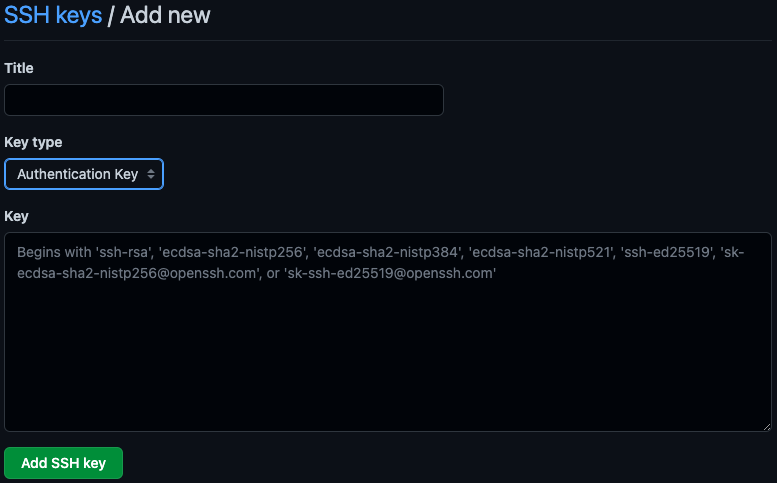
\includegraphics[width=.9\textwidth]{github-2}
\caption{Form Penambahan SSH-Key di GitHub}
\label{gam:tambah-ssh}
\end{figure}

Untuk menguji bahwa penambahan SSH-Key telah berhasil coba lakukan {\tt git push} untuk repositori laporan practice big data dari akun masing-masing. Untuk lebih jelasnya tentang GIT dapat membaca catatan pada link berikut \url{https://muhdavi.github.io/learn-git/}.
\end{enumerate}

\begin{comment}
\begin{figure}[!ht]
\centering
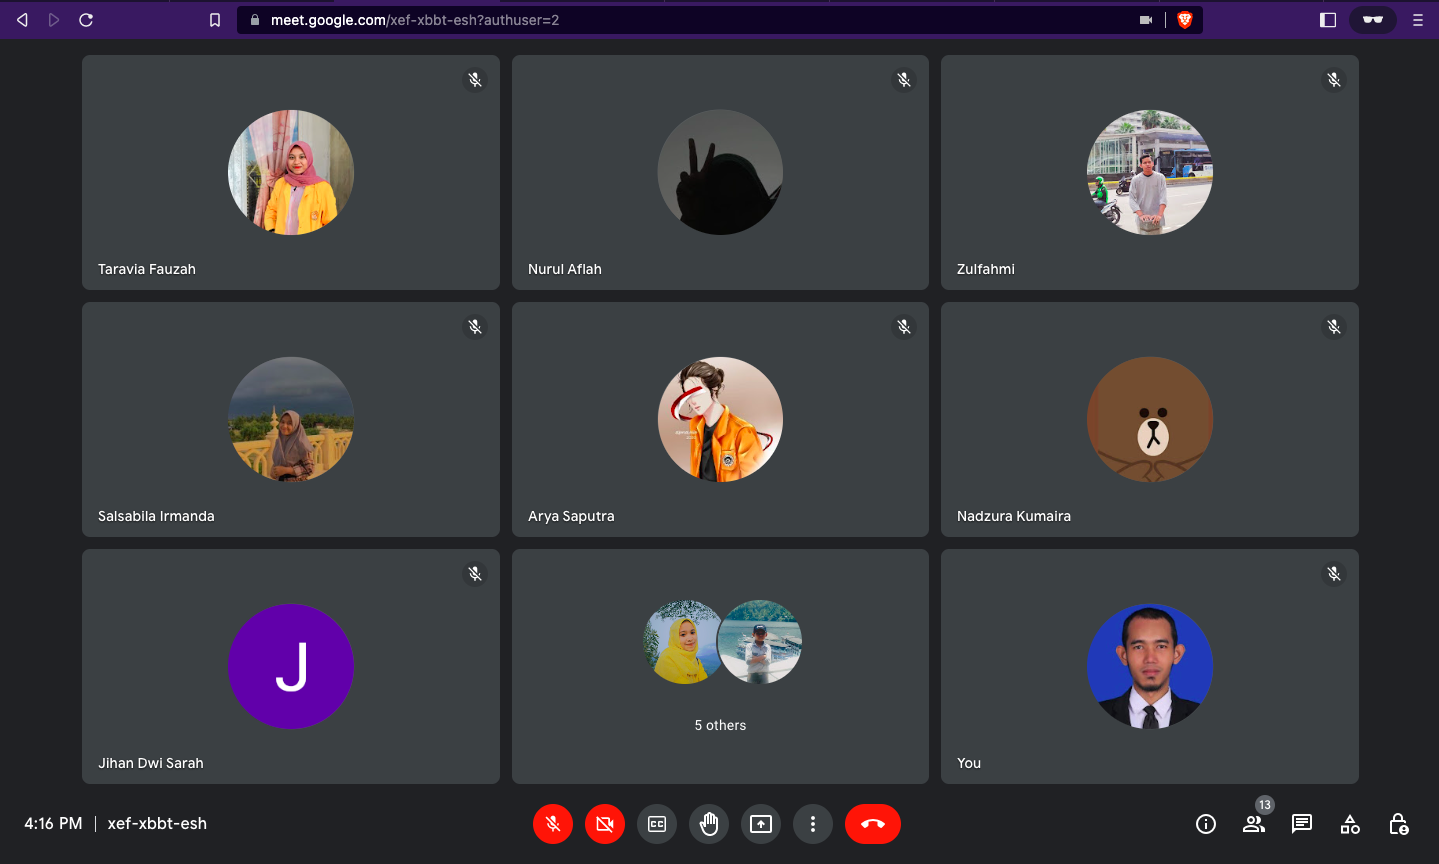
\includegraphics[width=.9\textwidth]{24-11-2022}
\caption{Perkuliahan Daring via Google Meet}
\label{gam:perkuliahan-24-11}
\end{figure}

\vspace*{-.5cm}
\hrulefill

%%%%%%%%%%%%%%%%%%%%%%%%%%%%%%%%%%%%%%%%%%%%%%%%%%%%%%%%
\clearpage
\newday{\#3 - 22 September 2022}
\newday{\#4 - 24 November 2022 menggantikan 29 September 2022}
\newday{\#5 - 25 November 2022 menggantikan 6 Oktober 2022}

\newthought{Instalasi dan Konfigurasi GIT dengan GitHub - Lanjutan}

Mahasiswa yang sudah berhasil konfigurasi Git dengan GitHub dan melakukan {\tt Pull Request}:
\begin{multicols}{2}
\begin{enumerate}
\item Rizki Ilhami
\item Rauzatinur Syah $\star$
\item Taravia Fauzah
\item Resha Russita $\star$
\item Nurani Harum Fardaniah $\star$
\item Adinda Awaliah $\star$
\item Salsabila Irmanda $\star$
\item M. Ikhsan
\item Jihan Dwi Sarah $\star$
\item Cut Opy Mandalisa $\star$
\item Zulfahmi
\item Muhammad Munawir
\item Nuraula Tafiza
\item Muhammad Ikrammullah
\item Nadzura Kumaira
\item Adjie Yusmunandar
\item Nurul Aflah
\item Arya Saputra
\item Faiza Yuwafiqi
\item Siti Hajar Al Zahra
\item Syarfani Akbar
\end{enumerate}
\end{multicols}

\begin{figure}[!ht]
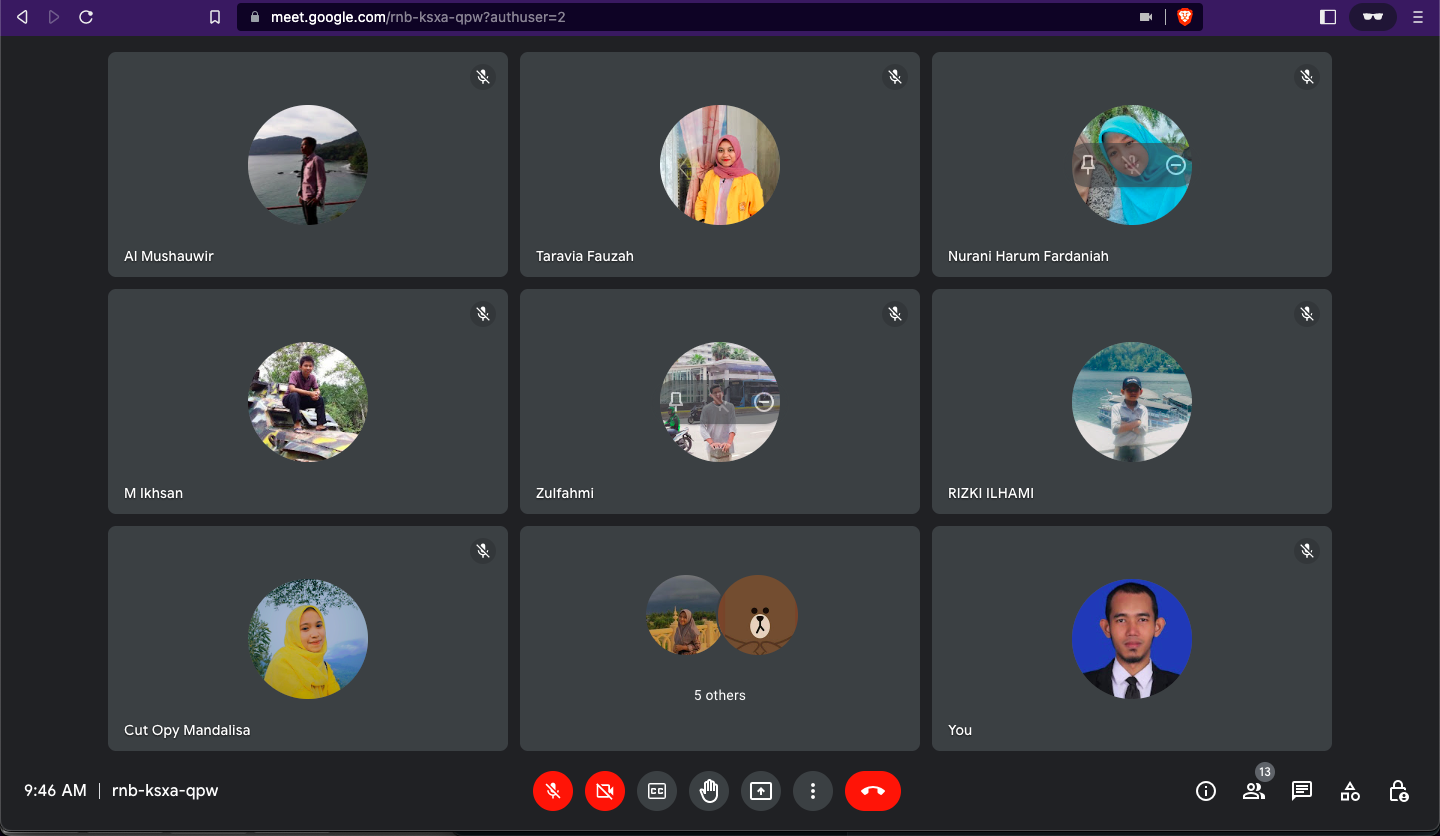
\includegraphics[width=\textwidth]{25-11-2022}
\caption{Perkuliahan Daring via Google Meet}
\label{gam:perkuliahan-25-11}
\end{figure}

\vspace*{-.5cm}
\hrulefill


%%%%%%%%%%%%%%%%%%%%%%%%%%%%%%%%%%%%%%%%%%%%%%%%%%%%%%%%
\clearpage
\newday{\#6 - 1 Desember 2022 menggantikan 13 Oktober 2022
\footnote{Mahasiswa yang hadir:
\begin{enumerate}
\item Adinda Awaliah
\item Arya Saputra $\oplus$
\item Cut Opy Mandalisa
\item Jihan Dwi Sarah
\item M. Ikhsan
\item Muhammad Ikrammullah
\item Muhammad Munawir
\item Nadzura Kumaira
\item Nurani Harum Fardaniah
\item Rauzatinur Syah
\item Resha Russita
\item Rizki Ilhami
\item Salsabila Irmanda
\item Syarfani Akbar
\item Taravia Fauzah
\item Zulfahmi
\end{enumerate}}}
\end{comment}

\newthought{Instalasi Apache Hadoop}

Pada pertemuan kedua ini kegiatan yang dilakukan adalah menginstall Apache Hadoop pada \textit{environment} yang telah dibuat pada pertemuan sebelumnya. Untuk menginstall Apache Hadoop dapat mengikut langkah-langkah berikut ini:

\begin{enumerate}
\item Membuat Group dan User Baru
\begin{itemize}
\item Membuat group
\begin{lstlisting}[language=Terminal]
 sudo addgroup hadoop
\end{lstlisting}

\item Membuat User Baru dan Menambahkan ke Group
\begin{lstlisting}[language=Terminal]
 sudo adduser -ingroup hadoop hdfs
\end{lstlisting}

\item Ubah Hak Akses
\begin{lstlisting}[language=Terminal]
 sudo visudo
\end{lstlisting}

\item Tambahkan Kode
\begin{lstlisting}
 hdfs	ALL=(ALL:ALL) ALL
\end{lstlisting}

\item Ganti ke User Baru
\begin{lstlisting}[language=Terminal]
 su - hdfs
\end{lstlisting}
\end{itemize}

\item Install Java
\begin{lstlisting}[language=Terminal]
 sudo apt update
 sudo apt install openjdk-8-jdk -y
\end{lstlisting}


\item Verifikasi Hasil Instalasi Java
\begin{lstlisting}[language=Terminal]
 java -version
\end{lstlisting}

Jika instalasi java berhasil tanpa ada bug atau error maka akan menampilkan hasil seperti pada Gambar \ref{gam:java-version}.

\begin{figure}
\setlength{\belowcaptionskip}{-10pt}
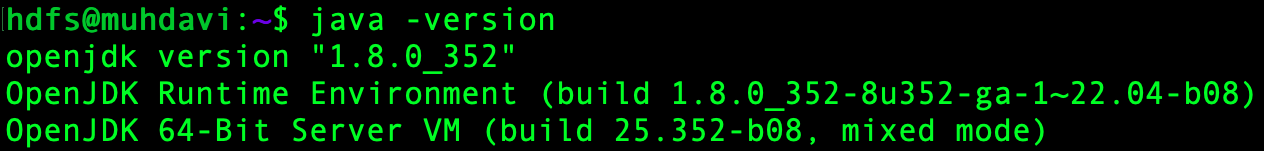
\includegraphics[width=\textwidth]{java-version}
\caption{Versi Java yang Terinstall}
\label{gam:java-version}
\end{figure}

\item Setting SSH
\begin{itemize}
\item Uninstall OpenSSH
\begin{lstlisting}[language=Terminal]
 sudo apt remove openssh-server openssh-client
\end{lstlisting}

\item Install OpenSSH Baru
\begin{lstlisting}[language=Terminal]
 sudo apt update
 sudo apt install openssh-server openssh-client
 sudo ufw allow 22
 sudo systemctl restart ssh
 sudo apt install ssh
 sudo apt install rsync
\end{lstlisting}

\item Generate Key
\begin{lstlisting}[language=Terminal]
 ssh-keygen -t dsa -P '' -f /home/hdfs/.ssh/id_dsa
 cat /home/hdfs/.ssh/id_dsa.pub >> /home/hdfs/.ssh/authorized_keys
 ssh-keygen -t rsa
\end{lstlisting}

\item Coba Masuk via SSH
\begin{lstlisting}[language=Terminal]
 ssh localhost
\end{lstlisting}

\item Jika masih harus memasukkan password, lanjutkan langakh berikut.
\begin{lstlisting}[language=Terminal]
 ssh-keygen -t rsa
 cat /home/hdfs/.ssh/id_rsa.pub >> /home/hdfs/.ssh/authorized_keys
 chmod og-wx /home/hdfs/.ssh/authorized_keys
 sudo apt update
\end{lstlisting}

\item Coba Masuk via SSH Lagi
\begin{lstlisting}[language=Terminal]
 ssh localhost
\end{lstlisting}

\item Jika sudah berhasil, keluar dengan perintah {\tt exit}
\begin{lstlisting}[language=Terminal]
 exit
\end{lstlisting}
\end{itemize}

\item Download Apache Hadoop
\begin{lstlisting}[language=Terminal]
 wget https://dlcdn.apache.org/hadoop/common/hadoop-3.3.4/hadoop-3.3.4.tar.gz
\end{lstlisting}

\item Ekstrak Apache Hadoop
\begin{lstlisting}[language=Terminal]
 tar -xzvf hadoop-3.3.4.tar.gz 
\end{lstlisting}

\begin{itemize}
\item x $\Rightarrow$ ekstrak file arsip.
\item z $\Rightarrow$ filter file arsip melalui gzip.
\item v $\Rightarrow$ menampilkan proses.
\item f $\Rightarrow$ nama file arsip.
\end{itemize}

\item Pindahkan hasil ekstraksi ke {\tt /usr/local/}
\begin{lstlisting}[language=Terminal]
 sudo mv hadoop-3.3.4 /usr/local/hadoop
\end{lstlisting}

\item Ubah Hak Akses {\tt /usr/local/hadoop}
\begin{lstlisting}[language=Terminal]
 sudo chown -R hdfs:hadoop /usr/local/hadoop
 sudo chmod -R 777 /usr/local/hadoop
\end{lstlisting}

\item Edit file {\tt sysctl.conf} untuk Disable IPV6
\begin{itemize}
\item Buka file {\tt sysctl.conf}
\begin{lstlisting}[language=Terminal]
 sudo nano /etc/sysctl.conf
\end{lstlisting}

\item Tambahkan Kode
\begin{lstlisting}[language=Bash]
net.ipv6.conf.all.disable_ipv6=1
net.ipv6.conf.lo.disable_ipv6=1
net.ipv6.conf.default_ipv6=1
\end{lstlisting}
\end{itemize}

\item Edit file {\tt hadoop-env.sh}
\begin{lstlisting}[language=Terminal]
 cd /usr/local/hadoop/etc/hadoop
 sudo nano hadoop-env.sh
\end{lstlisting}

\begin{lstlisting}[language=Bash]
export JAVA_HOME=/usr/lib/jvm/java-8-openjdk-amd64
export HADOOP_OPTS=-Djava.net.preferIPv4Stack=true
export HADOOP_HOME_WARN_SUPPRESS="TRUE"
export HADOOP_ROOT_LOGGER="WARN"
\end{lstlisting}

\item Menambahkan Hadoop ke {\tt .bashrc}
\begin{lstlisting}[language=Terminal]
 sudo nano $\sim$/.bashrc
\end{lstlisting}

\begin{lstlisting}[language=Bash]
# Hadoop Location
export HADOOP_HOME=/usr/local/hadoop
export HADOOP_CONF_DIR=/usr/local/hadoop/etc/hadoop
export HADOOP_MAPRED_HOME=/usr/local/hadoop
export HADOOP_COMMON_HOME=/usr/local/hadoop
export HADOOP_HDFS_HOME=/usr/local/hadoop
export YARN_HOME=/usr/local/hadoop
export PATH=$PATH:/usr/local/hadoop/bin
export PATH=$PATH:/usr/local/hadoop/sbin

# Hadoop Native Location
export HADOOP_COMMON_LIB_NATIVE_DIR=$HADOOP_HOME/lib/native
export HADOOP_OPTS="$HADOOP_OPTS -Djava.library.path=$HADOOP_HOME/lib/native"
export LD_LIBRARY_PATH=$HADOOP_HOME/lib/native
\end{lstlisting}

\begin{lstlisting}[language=Terminal]
 source /home/hdfs/.bashrc
\end{lstlisting}

\item Verifikasi Hasil Instalasi Hadoop
\begin{lstlisting}[language=Terminal]
 hadoop version
\end{lstlisting}

Jika instalasi hadoop berhasil, maka ketika mengecek versi hadoop akan muncul seperti yang diperlihatkan pada Gambar \ref{gam:hadoop-version}.
\begin{figure}[!ht]
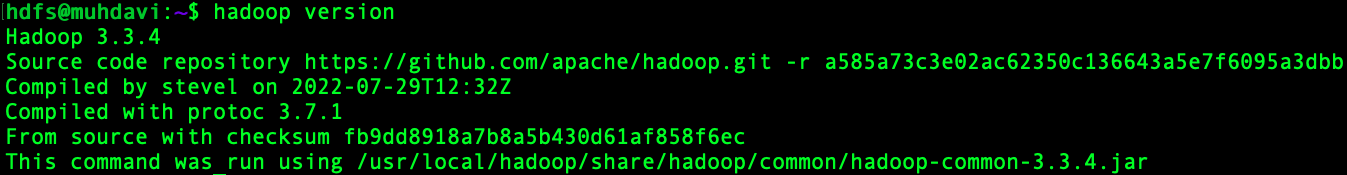
\includegraphics[width=\textwidth]{hadoop-version}
\caption{Versi Hadoop Terinstall 3.3.4}
\label{gam:hadoop-version}
\end{figure}
\end{enumerate}
 
\hrulefill

%%%%%%%%%%%%%%%%%%%%%%%%%%%%%%%%%%%%%%%%%%%%%%%%%%%%%%%%
\clearpage
\begin{comment}
\newday{\#7 - 2 Desember 2022 menggantikan 20 Oktober 2022
\footnote{Mahasiswa yang hadir:
\begin{enumerate}
\item Muhammad Munawir
\item Rizki Ilhami
\item Rauzatinur Syah
\item Salsabila Irmanda
\item Adjie Yusmunandar
\item Nurani Harum Fardaniah
\item Cut Opy Mandalisa
\item Resha Russita
\item Taravia Fauzah
\item Adinda Awaliah
\item Jihan Dwi Sarah
\item M. Ikhsan
\item Zulfahmi
\end{enumerate}}}
\end{comment}

\newthought{Konfigurasi Apache Hadoop}

Setelah selesai meng-install Hadoop, kita perlu konfigurasi beberapa file Hadoop agar memudahkan kita dalam memonitoring ekosistem Hadoop yang telah diinstall.

\begin{enumerate}
\item Konfigurasi File Hadoop \\
Beberapa file Hadoop yang perlu dikonfigurasi berada pada folder {\tt hadoop/etc/hadoop} seperti yang diperlihatkan pada Gambar \ref{gam:file-hadoop}. Konfigurasi file-file tersebut dapat menggunakan {\tt nano} diikuti nama file. Sisipkan kode konfigurasi diantara tag {\tt <configuration> $\cdots$ </configuration>}.

\begin{figure}[!ht]
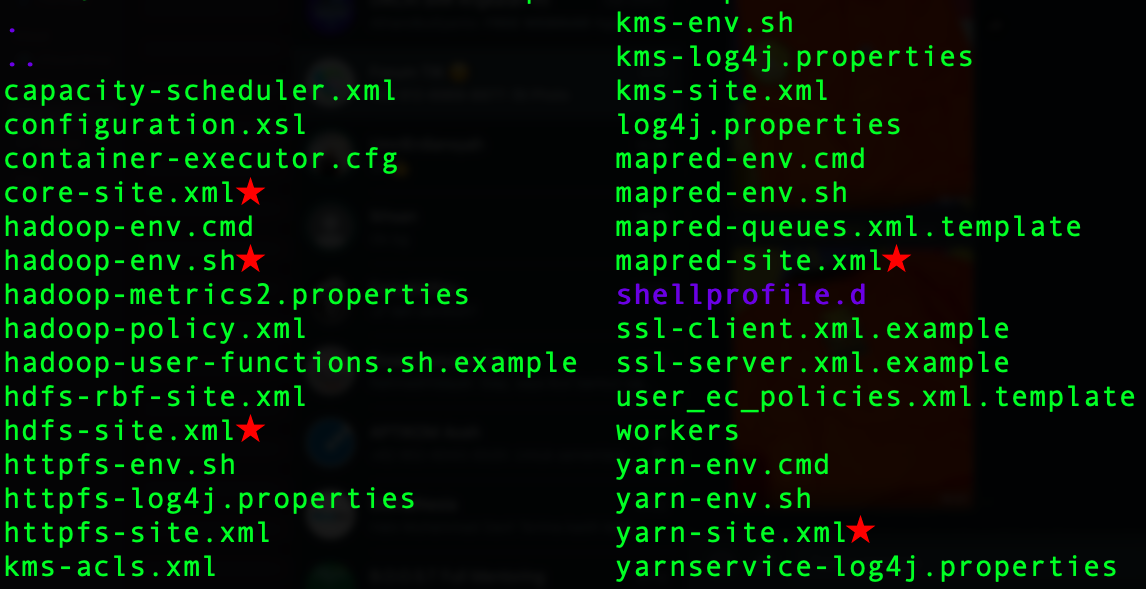
\includegraphics[width=\textwidth]{file-hadoop}
\caption{File Konfigurasi Hadoop}
\label{gam:file-hadoop}
\end{figure}

Berikut bebrapa file yang perlu dikonfigurasi dan lakukan dengan hati-hati serta teliti malalui perintah berikut:
\begin{lstlisting}[language=Terminal]
 cd /usr/local/hadoop/etc/hadoop
 sudo nano nama-file
\end{lstlisting}

\begin{itemize}

\item {\tt sudo nano core-site.xml}
\begin{lstlisting}[language=XML]
<property>
	<name>hadoop.tmp.dir</name>
	<value>/app/hadoop/tmp</value>
</property>
<property>
	<name>fs.default.name</name>
	<value>hdfs://localhost:9000</value>
</property>
\end{lstlisting}

\item {\tt sudo nano hdfs-site.xml}
\begin{lstlisting}[language=XML]
<property>
	<name>dfs.replication</name>
	<value>1</value>
</property>
<property>
	<name>dfs.namenode.name.dir</name>
	<value>file:/usr/local/hadoop/yarn_data/hdfs/namenode</value>
</property>
<property>
	<name>dfs.datanode.data.dir</name>
	<value>file:/usr/local/hadoop/yarn_data/hdfs/datanode</value>
</property>
\end{lstlisting}

\item {\tt sudo nano mapred-site.xml}
\begin{lstlisting}[language=XML]
<property>
	<name>mapred.framework.name</name>
	<value>yarn</value>
</property>
<property>
	<name>mapreduce.jobhistory.address</name>
	<value>localhost:10020</value>
</property>
\end{lstlisting}

\item {\tt sudo nano yarn-site.xml}
\begin{lstlisting}[language=XML]
<property>
	<name>yarn.nodemanager.aux-services</name>
	<value>mapreduce_shuffle</value>
</property>
<property>
	<name>yarn.nodemanager.aux-services.mapreduce.shuffle.class</name>
	<value>org.apache.hadoop.mapred.ShuffleHandler</value>
</property>
\end{lstlisting}
\end{itemize}

\item Membuat Folder Sementara (\textit{Temporary}) untuk HDFS
\begin{lstlisting}[language=Terminal]
 sudo mkdir -p /app/hadoop/tmp
 sudo chmod -R 777 /app/hadoop/tmp
 sudo chown -R hdfs:hadoop /app/hadoop/tmp
\end{lstlisting}

\item Membuat Folder {\tt namenode} dan {\tt datanode}
\begin{lstlisting}[language=Terminal]
 sudo mkdir -p /usr/local/hadoop/yarn\_data/hdfs/namenode
 sudo mkdir -p /usr/local/hadoop/yarn\_data/hdfs/datanode
 sudo chown -R hdfs:hadoop /usr/local/hadoop/yarn\_data/hdfs/namenode
 sudo chown -R hdfs:hadoop /usr/local/hadoop/yarn\_data/hdfs/datanode
 sudo chmod -R 777 /usr/local/hadoop/yarn\_data/hdfs/namenode
 sudo chmod -R 777 /usr/local/hadoop/yarn\_data/hdfs/datanode
\end{lstlisting}

\item Jalankan Perintah Format HDFS
\begin{lstlisting}[language=Terminal]
 hdfs namenode -format
\end{lstlisting}

\item Jalankan Hadoop Service
\begin{lstlisting}[language=Terminal]
 start-dfs.sh
 start-yarn.sh
\end{lstlisting}

\item Cek Hadoop Service
\begin{itemize}
\item Jalankan perintah {\tt jps}
\item Akses melalui web browser dengan alamat \url{http://localhost:9870}\footnote{Seperti yang diperlihatkan pada Gambar \ref{gam:namenode}} atau \url{http://localhost:8088}\footnote{Seperti yang diperlihatkan pada Gambar \ref{gam:resourcemanager}}.
\end{itemize}

\begin{figure}[!ht]
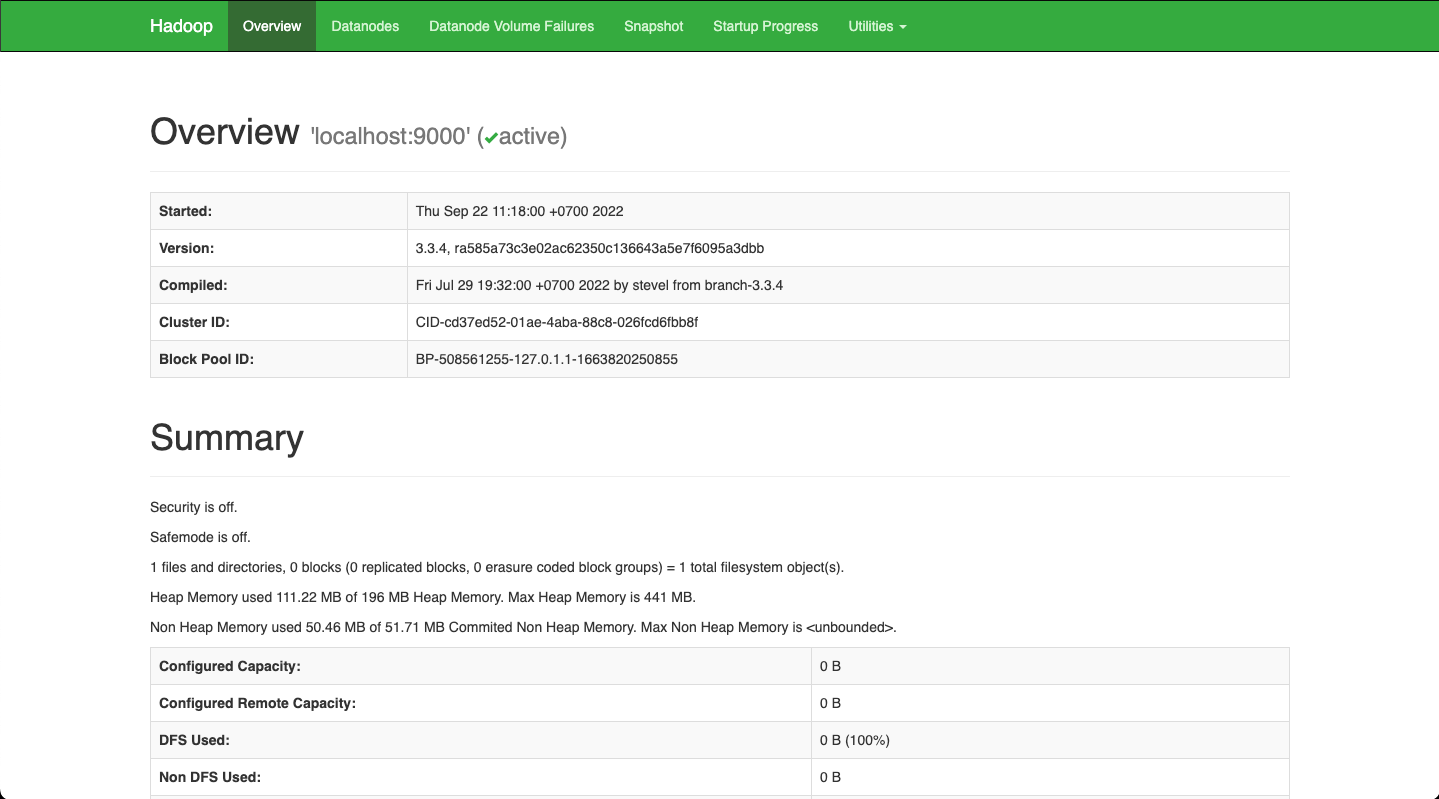
\includegraphics[width=\textwidth]{namenode}
\label{gam:namenode}
\end{figure}
\vspace*{-.7cm}
\begin{figure}[!ht]
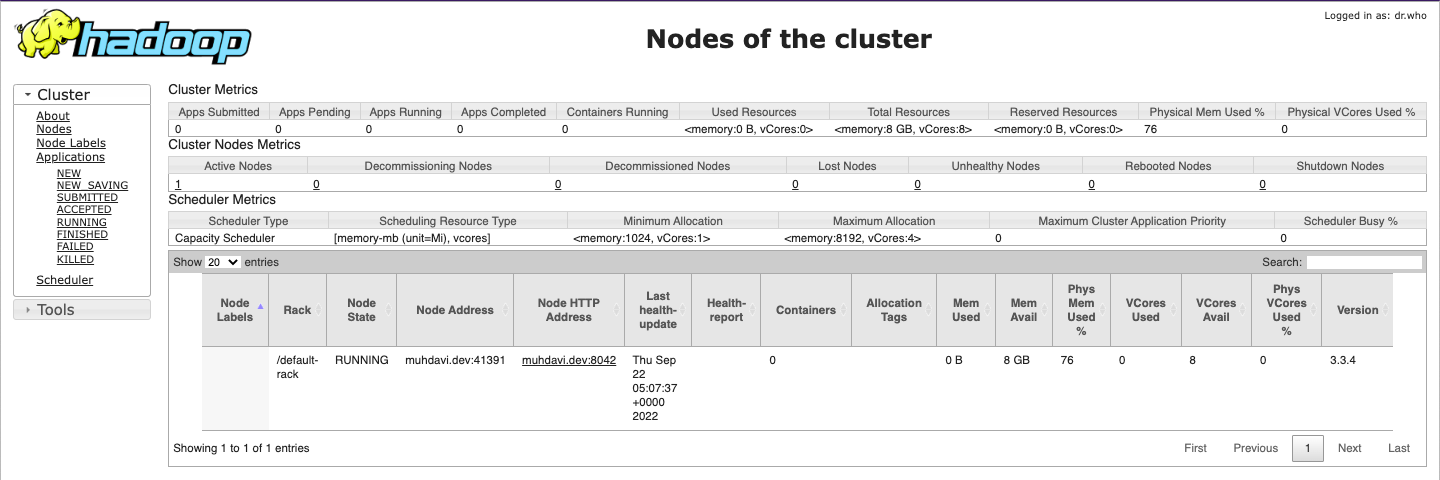
\includegraphics[width=\textwidth]{resourcemanager}
\caption{Resource Manager Hadoop}
\label{gam:resourcemanager}
\end{figure}

\vspace*{-.7cm}
\item Hentikan Hadoop Service
\begin{itemize}
\item Hentikan Service Tertentu
\begin{lstlisting}[language=Terminal]
 stop-dfs.sh
\end{lstlisting} 
atau
\begin{lstlisting}[language=Terminal]
 stop-yarn.sh
\end{lstlisting}
 
\item Hentikan Semua Service
\begin{lstlisting}[language=Terminal]
 stop-all.sh
\end{lstlisting}
\end{itemize}
\end{enumerate}
% mounting data shared folder
% sudo mount -t vboxsf share /mnt/share

\vspace*{.1cm}
\hrulefill

\begin{comment}
%%%%%%%%%%%%%%%%%%%%%%%%%%%%%%%%%%%%%%%%%%%%%%%%%%%%%%%%
\clearpage
\newday{\#8 - 8 Desember 2022 menggantikan 3 November 2022
\footnote{Mahasiswa yang hadir:
\begin{enumerate}
\item Adinda Awaliah
\item Adjie Yusmunandar
%\item Arya Saputra
\item Cut Opy Mandalisa
%\item Faiza Yuwafiqi
\item Jihan Dwi Sarah
\item M. Ikhsan
\item Muhammad Ikrammullah
\item Muhammad Munawir
%\item Nadzura Kumaira
\item Nurani Harum Fardaniah
%\item Nuraula Tafiza
%\item Nurul Aflah
\item Rauzatinur Syah
\item Resha Russita
\item Rizki Ilhami
\item Salsabila Irmanda
%\item Siti Hajar Al Zahra
%\item Syarfani Akbar
\item Taravia Fauzah
\item Zulfahmi
\end{enumerate}}}

\newday{\#9 - 9 Desember 2022 menggantikan 10 November 2022
\footnote{Mahasiswa yang hadir:
\begin{enumerate}
\item Adinda Awaliah
\item Adjie Yusmunandar
%\item Arya Saputra
\item Cut Opy Mandalisa
%\item Faiza Yuwafiqi
\item Jihan Dwi Sarah
\item M. Ikhsan
%\item Muhammad Ikrammullah
\item Muhammad Munawir
%\item Nadzura Kumaira
\item Nurani Harum Fardaniah
%\item Nuraula Tafiza
%\item Nurul Aflah
\item Rauzatinur Syah
\item Resha Russita
\item Rizki Ilhami
\item Salsabila Irmanda
%\item Siti Hajar Al Zahra
%\item Syarfani Akbar
\item Taravia Fauzah
\item Zulfahmi
\end{enumerate}}}

\newthought{Instalasi Apache Hadoop - Lanjutan}

\noindent
Mahasiswa yang sudah berhasil install Apache Hadoop:
\begin{multicols}{2}
\begin{enumerate}
\item Taravia Fauzah
\item Jihan Dwi Sarah
\item Salsabila Irmanda
\item Rauzatinur Syah
\item Resha Russita
\item Nurani Harum Fardaniah
\item Rizki Ilhami
\item Cut Opy Mandalisa
\end{enumerate}
\end{multicols}

\noindent
Mahasiswa yang sedang progress install Apache Hadoop :
\begin{multicols}{2}
\begin{enumerate}
\item Muhammad Ikrammullah
\item Zulfahmi
\item M. Ikhsan
\item Adjie Yusmunandar
\item Muhammad Munawir
\item Adinda Awaliah
\item Arya Saputra
\item Faiza Yuwafiqi
\item Nadzura Kumaira
\item Nuraula Tafiza
\item Nurul Aflah
\item Siti Hajar Al Zahra
\item Syarfani Akbar
\end{enumerate}
\end{multicols}

\hrulefill

%%%%%%%%%%%%%%%%%%%%%%%%%%%%%%%%%%%%%%%%%%%%%%%%%%%%%%%%
\clearpage
\newday{\#10 - 15 Desember 2022 menggantikan 10 November 2022
\footnote{Mahasiswa yang hadir:
\begin{enumerate}
\item Adinda Awaliah
\item Adjie Yusmunandar
\item Arya Saputra
\item Cut Opy Mandalisa
\item Faiza Yuwafiqi
\item Jihan Dwi Sarah
\item M. Ikhsan
\item Muhammad Ikrammullah
\item Muhammad Munawir
\item Nadzura Kumaira
\item Nurani Harum Fardaniah
%\item Nuraula Tafiza
\item Nurul Aflah
\item Rauzatinur Syah
\item Resha Russita
\item Rizki Ilhami
\item Salsabila Irmanda
%\item Siti Hajar Al Zahra
%\item Syarfani Akbar
\item Taravia Fauzah
%\item Zulfahmi
\end{enumerate}}}
\end{comment}

\newthought{Program WordCount bawaan Hadoop}

Jika sudah selesai malakukan instalasi Hadoop, maka dapat mencoba program bawaan Hadoop untuk memahami bagaimana proses dan cara kerja Hadoop dalam memproses data input hingga menghasilkan sebuah output. Salah satu program yang sudah disediakan oleh Hadoop adalah WordCount, yaitu program menghitung jumlah kata dalam data input yang dibarikan. Silahkan ikuti langkah-langkah berikut ini untuk mengetahui cara penggunaan program WordCount.

\begin{enumerate}
\item Jalankan Hadoop Service
\begin{lstlisting}[language=Terminal]
 start-dfs.sh
 yarn-dfs.sh
\end{lstlisting}

\item Buat folder input di HDFS
\begin{lstlisting}[language=Terminal]
 hadoop fs -mkdir /input
\end{lstlisting}

\item Buat file baru dengan nama dan data berikut
\begin{lstlisting}[language=Terminal]
 sudo nano dataWordCount.txt
\end{lstlisting}

\begin{lstlisting}[language=CSV, label={lst:data-wordcount}, caption=Data WorkCount]
AdindaAwaliah, SMA_N_1_Lhokseumawe, Cunda
AdjieYusmunandar, SMK_N_1_Lhokseumawe, Paloh_Lada
AryaSaputra, SMK_N_2_Lhokseumawe, Blang_Pulo
CutOpyMandalisa, SMA_N_1_Syamtalira_Bayu, Bayu
FaizaYuwafiqi, SMK_N_3_Lhokseumawe, Panggoi
JihanDwiSarah, SMA_N_1_Lhokseumawe, Panggoi
M.Ikhsan, SMK_N_1_Simpang_Kiri, Subulussalam
MuhammadIkrammullah, SMK_N_1_Lhokseumawe, Banda_Sakti
MuhammadMunawir, SMK_N_1_Lhoksukon, Karing_Meurah_Mulia
NadzuraKumaira, SMK_N_2_Lhokseumawe, Keude_Aceh
NuraniHarumFardaniah, SMK_N_1_Lhoksukon, Buket_Hagu
NuraulaTafiza, SMK_N_1_Lhoksukon, Alue_Buket
NurulAflah, MAS_Syamsuddhuha, Glp._Sulu_Barat
RauzatinurSyah, MAS_Misbahul_Ulum, Geudong
ReshaRussita, SMA_N_1_Lhokseumawe, Alue_Awe
RizkiIlhami, SMK_N_1_Lhoksukon, Lapang
SalsabilaIrmanda, MAS_Misbahul_Ulum, Alue_Awe
SitiHajarAlZahra, MAN_4_Aceh_Utara, Blang_Jruen
SyarfaniAkbar, SMK_N_1_Lhokseumawe, Uten_Bayi
TaraviaFauzah, SMA_N_1_Dewantara, Blang_Naleung_Mameh
Zulfahmi, SMK_N_1_Lhokseumawe, Kuta_Makmur
\end{lstlisting}

\item Pindahkan file {\tt dataWordCount.txt} ke folder input di HDFS
\begin{lstlisting}[language=Terminal]
 hadoop fs -put dataWordCount.txt /input
\end{lstlisting}

\item Jalankan program WordCount
\begin{lstlisting}[language=Terminal]
 hadoop jar /usr/local/hadoop/share/hadoop/mapreduce/hadoop-mapreduce-examples-3.3.4.jar wordcount /input/dataWordCount.txt /output
\end{lstlisting} 
%hadoop jar /usr/local/hadoop/share/hadoop/mapreduce/hadoop-mapreduce-examples-3.2.0.jar wordcount /input/ /output2 -> untuk semua file dari folder input

\item Cek Hasil
\begin{lstlisting}[language=Terminal]
 hadoop fs -ls /output
\end{lstlisting} 

\item Lihat Hasil
\begin{lstlisting}[language=Terminal]
 hadoop fs -cat /output/part-r-00000
\end{lstlisting} 
\end{enumerate}

\newthought{Tugas Praktikum} \\
Screenshot hasil dari langkah 6 dan 7 dan masukkan ke dalam laporan. Kumpulkan melalui {\tt pull requests} dengan format pesan "\textit{Laporan dd-mm-yyyy an. Nama}".

\hrulefill

%%%%%%%%%%%%%%%%%%%%%%%%%%%%%%%%%%%%%%%%%%%%%%%%%%%%%%%%
\clearpage
\begin{comment}
\newday{\#11 - 16 Desember 2022 menggantikan 17 November 2022
\footnote{Mahasiswa yang hadir:
\begin{enumerate}
\item Adinda Awaliah
\item Adjie Yusmunandar
%\item Arya Saputra
%\item Cut Opy Mandalisa
\item Faiza Yuwafiqi
\item Jihan Dwi Sarah
\item M. Ikhsan
%\item Muhammad Ikrammullah
%\item Muhammad Munawir
%\item Nadzura Kumaira
\item Nurani Harum Fardaniah
\item Nuraula Tafiza
\item Nurul Aflah
\item Rauzatinur Syah
\item Resha Russita
\item Rizki Ilhami
\item Salsabila Irmanda
%\item Siti Hajar Al Zahra
%\item Syarfani Akbar
\item Taravia Fauzah
\item Zulfahmi
\end{enumerate}}}
\end{comment}

\newthought{Program WordCount dengan Java}

Pada pertemuan sebelumnya telah mencoba program WordCount bawaan Hadoop. Jika dengan program bawaan Hadoop sudah dapat mendapatkan hasil, artinya Hadoop kita sudah bisa digunakan untuk menjalankan program. Ikuti beberapa langkah berikut untuk memberikan pemahaman bagaimana proses membuat program, menyiapkan data, meng-compile program hingga menjalankan program dan memperoleh hasilnya.

\begin{enumerate}
\item Pastikan Hadoop Service sudah berjalan
\item Pastikan data input pada pertemuan sebelumnya masih tersedia di HDFS
\begin{lstlisting}[language=Terminal]
 hadoop fs -ls /input
\end{lstlisting}

\item Buat file baru dengan nama dan kode berikut
\begin{lstlisting}[language=Terminal]
 sudo nano WordCount.java
\end{lstlisting} 
\lstinputlisting[caption=Code WordCount Java, label={lst:wordcount-java}, language=Java]{code/wordcount-java.java}
% https://github.com/muhdavi/kode-practice-big-data/blob/main/WordCountJava/src/main/java/WordCount.java

\item Buat classpath
\begin{lstlisting}[language=Terminal]
 export HADOOP\_CLASSPATH=\$(\$HADOOP\_HOME/bin/hadoop classpath)
\end{lstlisting} 

\item Buat folder baru untuk menampung hasil \textit{compile} program java dan ubah hak aksesnya
\begin{lstlisting}[language=Terminal]
 sudo mkdir JavaCompiled
 sudo chmod -R 777 JavaCompiled
\end{lstlisting}

\item Compile file WordCount.java
\begin{lstlisting}[language=Terminal]
 javac -classpath \$HADOOP\_CLASSPATH -d JavaCompiled/WordCount.java
\end{lstlisting}

\item Mengubah file menjadi executable .jar
\begin{lstlisting}[language=Terminal]
 jar -cvf WordCount.jar -C JavaCompiled/ .
\end{lstlisting}

\item Jalankan program WordCount
\begin{lstlisting}[language=Terminal]
 hadoop jar WordCount.jar WordCount /input/dataWordCount.txt /ResultWordCountJava
\end{lstlisting}

\item Cek Hasil
\begin{lstlisting}[language=Terminal]
 hadoop fs -ls /ResultWordCountJava
\end{lstlisting}

\item Lihat Hasil
\begin{lstlisting}[language=Terminal]
 hadoop fs -cat /ResultWordCountJava/part-r-00000
\end{lstlisting} 
\end{enumerate}

\newthought{Tugas Praktikum} \\
Screenshot hasil dari langkah 9 dan 10 serta masukkan ke dalam laporan. Kumpulkan melalui {\tt pull requests} dengan format pesan "\textit{Laporan dd-mm-yyyy an. Nama}".

\hrulefill

%%%%%%%%%%%%%%%%%%%%%%%%%%%%%%%%%%%%%%%%%%%%%%%%%%%%%%%%
\clearpage
\begin{comment}
\newday{\#12 - 22 Desember 2022 menggantikan 24 November 2022
\footnote{Mahasiswa yang hadir:
\begin{enumerate}
\item Adinda Awaliah
\item Adjie Yusmunandar
\item Arya Saputra
\item Cut Opy Mandalisa
%\item Faiza Yuwafiqi
\item Jihan Dwi Sarah
\item M. Ikhsan
%\item Muhammad Ikrammullah
\item Muhammad Munawir
\item Nadzura Kumaira
\item Nurani Harum Fardaniah
\item Nuraula Tafiza
\item Nurul Aflah
\item Rauzatinur Syah
\item Resha Russita
\item Rizki Ilhami
\item Salsabila Irmanda
\item Siti Hajar Al Zahra
\item Syarfani Akbar
\item Taravia Fauzah
\item Zulfahmi
\end{enumerate}}}
\end{comment}

\newthought{Instalasi Apache Spark (PySpark)}

\begin{enumerate}
\item Download Apache Spark
\begin{lstlisting}[language=Terminal]
 wget https://dlcdn.apache.org/spark/spark-3.3.1/spark-3.3.1-bin-hadoop3.tgz
\end{lstlisting}

\item Ekstrak Apache Spark
\begin{lstlisting}[language=Terminal]
 tar -xzvf spark-3.3.1-bin-hadoop3.tgz
\end{lstlisting}

\item Pindahkan hasil ekstraksi ke {\tt /usr/local/}
\begin{lstlisting}[language=Terminal]
 sudo mv spark-3.3.1-bin-hadoop3 /usr/local/spark
\end{lstlisting} 

\item Menambahkan Spark ke {\tt .bashrc}
\begin{lstlisting}[language=Terminal]
 sudo nano /home/hdfs/.bashrc
\end{lstlisting} 
\begin{lstlisting}[language=Bash, label={lst:bash-spark}, caption=Code Konfig Apaceh Spark]
# Spark Location
export SPARK_HOME=/usr/local/spark
export PATH=$PATH:$SPARK_HOME/bin:$SPARK_HOME/sbin
\end{lstlisting}
\begin{lstlisting}[language=Terminal]
 source $\sim$/.bashrc
\end{lstlisting}

\item Verifikasi Hasil Instalasi Spark
\begin{lstlisting}[language=Terminal]
 pyspark ---version
\end{lstlisting}

\begin{figure}[!ht]
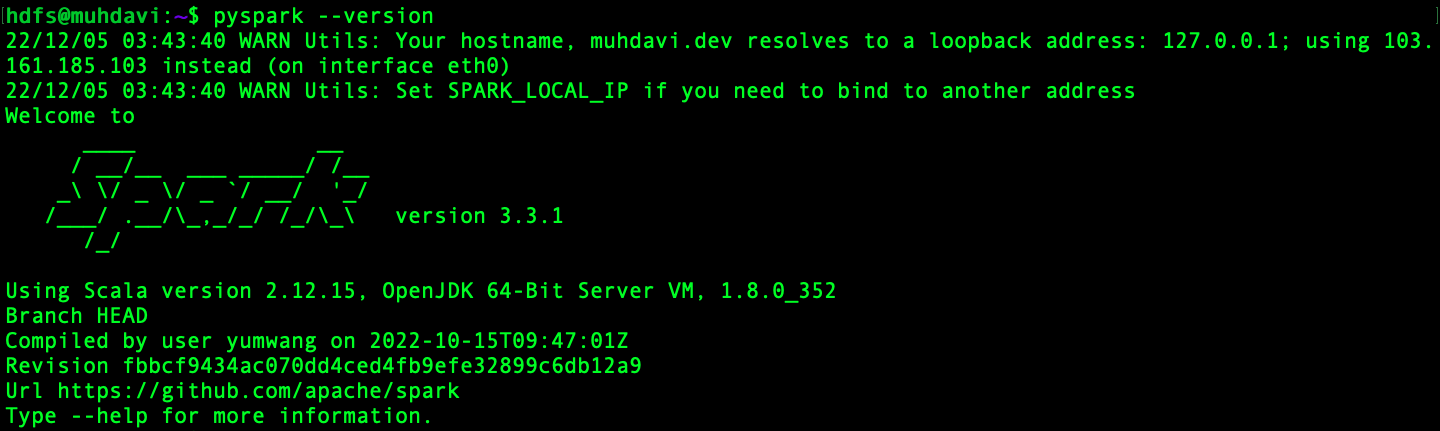
\includegraphics[width=\textwidth]{spark-version}
\caption{Versi Spark Terinstall 3.3.1 }
\label{gam:form-ssh}
\end{figure}

\item Jalankan Spark Service
\begin{lstlisting}[language=Terminal]
 start-master.sh
\end{lstlisting}

\item Hentikan Spark Service
\begin{lstlisting}[language=Terminal]
 stop-master.sh
\end{lstlisting} 
\end{enumerate}

\newthought{Tugas Praktikum} \\
Screenshot hasil dari langkah 5 dan masukkan ke dalam laporan. Kumpulkan melalui {\tt pull requests} dengan format pesan "\textit{Laporan dd-mm-yyyy an. Nama}".

\hrulefill

%%%%%%%%%%%%%%%%%%%%%%%%%%%%%%%%%%%%%%%%%%%%%%%%%%%%%%%%
\clearpage
\begin{comment}
\newday{\#13 - 23 Desember 2022 menggantikan 1 Desember 2022
\footnote{Mahasiswa yang hadir:
\begin{enumerate}
\item Adinda Awaliah
%\item Adjie Yusmunandar
%\item Arya Saputra
\item Cut Opy Mandalisa
\item Faiza Yuwafiqi
\item Jihan Dwi Sarah
\item M. Ikhsan
%\item Muhammad Ikrammullah
%\item Muhammad Munawir
%\item Nadzura Kumaira
\item Nurani Harum Fardaniah
%\item Nuraula Tafiza
%\item Nurul Aflah
\item Rauzatinur Syah
\item Resha Russita
\item Rizki Ilhami
\item Salsabila Irmanda
%\item Siti Hajar Al Zahra
%\item Syarfani Akbar
\item Taravia Fauzah
\item Zulfahmi
\end{enumerate}}}
\end{comment}

\newthought{Program WordCount dengan Python}

\begin{enumerate}
\item Pastikan Hadoop Service dan Spark Service berjalan
\item Pastikan data input pada pertemuan sebelumnya masih tersedia di HDFS
\item Buat folder baru untuk menyimpan file Python
\begin{lstlisting}[language=Terminal]
 sudo mkdir WordCountPython
\end{lstlisting}

\item Buat file baru dengan nama dan kode berikut
\begin{itemize}
\item {\tt map.py}
\begin{lstlisting}[language=Terminal]
 sudo nano WordCountPython/map.py
\end{lstlisting}
 
\lstinputlisting[caption=Code Map Python, label={lst:map-python}, language=Python]{code/map.py}
%{\tt wget https://raw.githubusercontent.com/muhdavi/kode-practice- big-data/main/WordCountPython/map.py}

\item {\tt reduce.py}
\begin{lstlisting}[language=Terminal]
 sudo nano WordCountPython/reduce.py
\end{lstlisting} 
\lstinputlisting[caption=Code Reduce Python, label={lst:reduce-python}, language=Python]{code/reduce.py}
%{\tt wget https://raw.githubusercontent.com/muhdavi/kode-practice- big-data/main/WordCountPython/reduce.py}
\end{itemize}

\item Ubah Hak Akses
\begin{lstlisting}[language=Terminal]
 sudo chmod +x -R WordCountPython/
\end{lstlisting}

\item Mencoba Program di Local
\begin{lstlisting}[language=Terminal]
 echo jangan heran jika orang cantik merasa jelek sementara orang yang jelek merasa cantik | WordCountPython/map.py | sort | WordCountPython/reduce.py
\end{lstlisting}

\item Jalankan Program menggunakan Hadoop
\begin{lstlisting}[language=Terminal]
 hadoop jar /usr/local/hadoop/share/hadoop/tools/lib/hadoop-streaming-3
 .3.4.jar -mapper /home/hdfs/WordCountPython/map.py -reducer /home/hdfs
 /WordCountPython/reduce.py -input /input/dataWordCount.txt -output /Re
 sultWordCountPython
\end{lstlisting}

\item Cek Hasil
\begin{lstlisting}[language=Terminal]
 hadoop fs -ls /ResultWordCountPython
\end{lstlisting}

\item Lihat Hasil 
\begin{lstlisting}[language=Terminal]
 hadoop fs -cat /ResultWordCountPython/part-00000
\end{lstlisting}

\end{enumerate}

\vspace*{-.5cm}
\newthought{Tugas Praktikum} \\
Screenshot hasil dari langkah 8 dan 9 serta masukkan ke dalam laporan. Kumpulkan melalui {\tt pull requests} dengan format pesan "\textit{Laporan dd-mm-yyyy an. Nama}".

\hrulefill

%%%%%%%%%%%%%%%%%%%%%%%%%%%%%%%%%%%%%%%%%%%%%%%%%%%%%%%%
\clearpage
%\newday{\#14 - 23 Desember 2022 menggantikan 8 Desember 2022}

\newthought{Program WordCount dengan PySpark}

\begin{enumerate}
\item Pastikan Hadoop Service dan Spark Service berjalan
\item Pastikan data input pada pertemuan sebelumnya masih tersedia di HDFS
\item Buat folder baru untuk menyimpan file Python
\begin{lstlisting}[language=Terminal]
 sudo mkdir WordCountPySpark
 cd WordCountPySpark
\end{lstlisting}

\item Buat file baru dengan nama dan kode berikut
\begin{lstlisting}[language=Terminal]
 sudo nano WordCount.py
\end{lstlisting} 
\lstinputlisting[caption=Code WordCount PySpark, label={lst:wordcount-pyspark}, language=Python]{code/wordcount-pyspark.py}

\item Jalankan Program menggunakan PySpark
\begin{lstlisting}[language=Terminal]
 spark-submit WordCount.py
\end{lstlisting}

\item Cek Hasil
\begin{lstlisting}[language=Terminal]
 hadoop fs -ls /ResultWordCountPyspark
\end{lstlisting}

\item Lihat Hasil
\begin{lstlisting}[language=Terminal]
 hadoop fs -cat /ResultWordCountPyspark/part-00000
\end{lstlisting} 
\end{enumerate}

\vspace*{-.5cm}
\newthought{Tugas Praktikum} \\
Screenshot hasil dari langkah 6 dan 7 serta masukkan ke dalam laporan. Kumpulkan melalui {\tt pull requests} dengan format pesan "\textit{Laporan dd-mm-yyyy an. Nama}".

\hrulefill

%%%%%%%%%%%%%%%%%%%%%%%%%%%%%%%%%%%%%%%%%%%%%%%%%%%%%%%%
\clearpage
%\newday{\#15 - Tugas Individu menggantikan 15 Desember 2022}

\newthought{Program Machine Learning dengan PySpark}

Berbeda dengan program sebelumnyan, program ini dijalankan satu-per-satu perintahnya di terminal PySpark. Ikutilah langkah-langkah berikut ini secara cermat dan teliti. Setiap perintah yang Anda kerjakan buat dokumentasi-nya dan Anda masukkan ke dalam Laporan dengan mengumpulkannya melalui GitHub dengan \textit{message "Laporan Tugas Mandiri a.n. Nama"}.

\begin{enumerate}
\item Pastikan Hadoop dan Spark berjalan
\item Pastikan package sudah tersedia
\begin{lstlisting}[language=Terminal]
 pip list
\end{lstlisting} 
\begin{multicols}{3}
\begin{itemize}
\item pandas
\item matplotlib
\item numpy
\item seaborn
\item scikit-learn
\end{itemize}
\end{multicols}

Jika package tersebut belum tersedia, install terlebih dahulu menggunakan {\tt pip}, misalnya {\tt pip install scikit-learn}.

\item Load Package
\begin{lstlisting}[language=Terminal]
 import numpy as np
 import pandas as pd
 import seaborn as sns
 import matplotlib.pyplot as plt
 from sklearn.datasets import load_iris
 from pyspark.sql import SparkSession
\end{lstlisting}

\item Load Data
\begin{lstlisting}[language=Terminal]
 data_iris = load_iris(as_frame=True)
 df = pd.DataFrame(data_iris.data, columns = data_iris.feature_names)
 spark_df = spark.createDataFrame(df)
 spark_df.show(5)
\end{lstlisting}

\item Menentukan nilai K dengan metode \textit{silhouette}
\begin{lstlisting}[language=Terminal]
from pyspark.ml.feature import VectorAssembler

assemble=VectorAssembler(inputCols=[
'sepal length (cm)',
'sepal width (cm)',
'petal length (cm)',
'petal width (cm)'],
outputCol = 'iris_features')

assembled_data=assemble.transform(spark_df)
assembled_data.show()
from pyspark.ml.clustering import KMeans
from pyspark.ml.evaluation import ClusteringEvaluator

silhouette_scores=[]

evaluator = ClusteringEvaluator(featuresCol='iris_features', 
metricName='silhouette', distanceMeasure='squaredEuclidean')

for K in range(|\color{white}2|,11):
	KMeans_=KMeans(featuresCol='iris_features', k=K)
	KMeans_fit=KMeans_.fit(assembled_data)
	KMeans_transform=KMeans_fit.transform(assembled_data)
	evaluation_score=evaluator.evaluate(KMeans_transform)
	silhouette_scores.append(evaluation_score)

fig, ax = plt.subplots(1,1, figsize=(10,8))
ax.plot(range(2,11), silhouette_scores)
ax.set_xlabel('Jumlah Cluster')
ax.set_ylabel('Hasil Silhouette')
plt.show()
\end{lstlisting}

\item Membangun Model \textit{K-Means Clustering}
\begin{lstlisting}[language=Terminal]
KMeans_=KMeans(featuresCol='iris_features', k=3)
KMeans_Model=KMeans_.fit(assembled_data)
KMeans_Assignments=KMeans_Model.transform(assembled_data)
\end{lstlisting}

\item Menampilkan Hasil \textit{Clustering} dengan PCA
\begin{lstlisting}[language=Terminal]
 from pyspark.ml.feature import PCA as PCAml
 pca = PCAml(k=2, inputCol="iris_features", outputCol="pca")
 pca_model = pca.fit(assembled_data)
 pca_transform = pca_model.transform(assembled_data)

 x_pca = np.array(pca_transform.rdd.map(lambda row: row.pca).collect())

 cluster_assignment = np.array(KMeans_Assignments.rdd.map(lambda row: ro
 w.prediction).collect()).reshape(-1,1)

 pca_data = np.hstack((x_pca,cluster_assignment))

 pca_df = pd.DataFrame(data=pca_data, columns=("1st_principal",
 "2nd_principal","cluster_assignment")) 

 sns.FacetGrid(pca_df,hue="cluster_assignment", height=6).map(plt.scatte
 r, '1st_principal', '2nd_principal').add_legend()

 plt.show()
\end{lstlisting}
\end{enumerate}

\hrulefill

%%%%%%%%%%%%%%%%%%%%%%%%%%%%%%%%%%%%%%%%%%%%%%%%%%%%%%%%
\clearpage
%\newday{\#16 - Tugas Kelompok menggantikan 22 Desember 2022}

\newthought{Program Machine Learning dengan PySpark}

Berdasarakn program sebelumnya yang telah Anda coba malalui Terminal PySpark, kerjakan tugas berikut secara berkelompok:

\begin{enumerate}
\item Buatlah program tersebut dalam bentuk file Python sehingga dapat dijalankan menggunakan {\tt spark-submit}.
\item Dokumentasikan hasil dan perubahan yang Anda lakukan untuk dimasukkan ke dalam laporan.
\item Kumpulkan laporan beserta file Python melalui GitHub dengan format \textit{message "Laporan Kelompok Nomor-Kelompok}".
\item Kumpulkan file Python didalam folder yang telah disediakan \textit{TugasKelompok}. Yang mengumpulkan cukup salah satu sebagai perwakilan/ketua kelompok.
\end{enumerate}

\hrulefill

\begin{center}
\noindent
\textbf{\textcolor{red}{Ingat!\\ Semua Tugas dan Laporan panling lambat dikumpulkan tanggal 5 Januari 2023.}}
\end{center}

\hrulefill

%%%%%%%%%%%%%%%%%%%%%%%%%%%%%%%%%%%%%%%%%%%%%%%%%%%%%%%%
\begin{comment}
\clearpage
\newthought{Rekap Progres Praktikum dan Penilaian\footnote{
Catatan Penilaian:
\begin{enumerate}
\item Arya Saputa: sering tidak masuk, laporan dikumpulkan pada saat perpanjangan waktu.
\item Siti Hajar Al Zahra: sering tidak masuk.
\item Syarfani Akbar dan Nuraula Tafiza: tidak mengumpulkan laporan.
\end{enumerate}}}

\begin{table}[!ht]
\vspace*{.5cm}
\hspace*{-1cm}
\centering
\begin{tabular}{cl|c|c|c|c|c|c|c|c|c} 
	& & 
	\multirow{9}{*}{\rotatebox{90}{\parbox[l]{3.3cm}{Install Hadoop}}} &
	\multirow{9}{*}{\rotatebox{90}{\parbox[l]{3.3cm}{WordCount Hadoop}}} &
	\multirow{9}{*}{\rotatebox{90}{\parbox[l]{3.3cm}{WordCount Java}}} & 
	\multirow{9}{*}{\rotatebox{90}{\parbox[l]{3.3cm}{Install Apache Spark}}} &
	\multirow{9}{*}{\rotatebox{90}{\parbox[l]{3.3cm}{WordCount Python}}} &
	\multirow{9}{*}{\rotatebox{90}{\parbox[l]{3.3cm}{WordCount PySpark}}} &
	\multirow{9}{*}{\rotatebox{90}{\parbox[l]{3.3cm}{Tugas Individu}}} &
	\multirow{9}{*}{\rotatebox{90}{\parbox[l]{3.3cm}{Tugas Kelompok}}} &
	\multirow{9}{*}{\rotatebox{90}{\parbox[l]{3.3cm}{Nilai Akhir}}} \\	
	& & & & & & & & & & \\
	& & & & & & & & & & \\
	& & & & & & & & & & \\
	& & & & & & & & & & \\
	& & & & & & & & & & \\
	& & & & & & & & & & \\
No 	& Nama 						& & & & & & & & & \\ \hline
1 	& Adinda Awaliah			& $\star$ & $\star$ & $\star$ & $\star$ & $\star$ & $\star$ & $\star$ & $\star$ & A \\ \hline
2 	& Adjie Yusmunandar			& $\star$ & $\star$ & & $\star$ & & & & $\star$ & B \\ \hline
3 	& Arya Saputra 				& $\star$ & $\star$ & $\star$ & $\star$ & $\star$ & $\star$ & & $\star$ & B \\ \hline
4 	& Cut Opy Mandalisa			& $\star$ & $\star$ & $\star$ & $\star$ & $\star$ & $\star$ & $\star$ & $\star$ & A \\ \hline
5 	& Faiza Yuwafiqi			& $\star$ & $\star$ & $\star$ & $\star$ & $\star$ & $\star$ & $\star$ & $\star$ & A \\ \hline
6 	& Jihan Dwi Sarah			& $\star$ & $\star$ & $\star$ & $\star$ & $\star$ & $\star$ & $\star$ & $\star$ & A \\ \hline
7 	& M. Ikhsan					& $\star$ & $\star$ & $\star$ & $\star$ & $\star$ & $\star$ & & & AB \\ \hline
8 	& Muhammad Ikrammullah		& $\star$ & $\star$ & $\star$ & $\star$ & $\star$ & $\star$ & $\star$ & & AB \\ \hline
9 	& Muhammad Munawir			& $\star$ & $\star$ & $\star$ & $\star$ & & & & & B \\ \hline
10 	& Nadzura Kumaira			& $\star$ & & & $\star$ & $\star$ & $\star$ & $\star$ & $\star$ & AB \\ \hline
11 	& Nurani Harum Fardaniah	& $\star$ & $\star$ & $\star$ & $\star$ & $\star$ & $\star$ & $\star$ & $\star$ & A\\ \hline
12 	& Nuraula Tafiza			& & & & & & & & $\star$ & BC\\ \hline
13 	& Nurul Aflah				& $\star$ & $\star$ & $\star$ & $\star$ & $\star$ & $\star$ & $\star$ & $\star$ & A \\ \hline
14 	& Rauzatinur Syah			& $\star$ & $\star$ & $\star$ & $\star$ & $\star$ & $\star$ & $\star$ & $\star$ & A \\ \hline
15 	& Resha Russita				& $\star$ & $\star$ & $\star$ & $\star$ & $\star$ & $\star$ & $\star$ & $\star$ & A \\ \hline
16 	& Rizki Ilhami				& $\star$ & $\star$ & $\star$ & $\star$ & $\star$ & $\star$ & $\star$ & $\star$ & A \\ \hline
17 	& Salsabila Irmanda			& $\star$ & $\star$ & $\star$ & $\star$ & $\star$ & $\star$ & $\star$ & $\star$ & A \\ \hline
18 	& Siti Hajar Al Zahra		& $\star$ & $\star$ & $\star$ & $\star$ & $\star$ & & & $\star$ & B \\ \hline
19 	& Syarfani Akbar			& & & & & & & & $\star$ & BC \\ \hline
20 	& Taravia Fauzah			& $\star$ & $\star$ & $\star$ & $\star$ & $\star$ & $\star$ & $\star$ & $\star$ & A \\ \hline
21 	& Zulfahmi					& $\star$ & $\star$ & $\star$ & $\star$ & $\star$ & $\star$ & & & AB \\ \hline
\multicolumn{2}{c|}{Perbandingan}		& 
$\frac{19}{2}$ &
$\frac{18}{3}$ &
$\frac{17}{4}$ &
$\frac{19}{2}$ &
$\frac{17}{4}$ &
$\frac{16}{5}$ &
$\frac{13}{8}$ &
$\frac{17}{4}$ &
$\frac{\frac{11}{4}}{\frac{4}{2}}$ \\
\end{tabular}
\end{table}

%\hrulefill

%%%%%%%%%%%%%%%%%%%%%%%%%%%%%%%%%%%%%%%%%%%%%%%%%%%%%%%%

\footnote{Mahasiswa yang hadir:
\begin{enumerate}
\item Adinda Awaliah
\item Adjie Yusmunandar
\item Arya Saputra
\item Cut Opy Mandalisa
\item Faiza Yuwafiqi
\item Jihan Dwi Sarah
\item M. Ikhsan
\item Muhammad Ikrammullah
\item Muhammad Munawir
\item Nadzura Kumaira
\item Nurani Harum Fardaniah
\item Nuraula Tafiza
\item Nurul Aflah
\item Rauzatinur Syah
\item Resha Russita
\item Rizki Ilhami
\item Salsabila Irmanda
\item Siti Hajar Al Zahra
\item Syarfani Akbar
\item Taravia Fauzah
\item Zulfahmi
\end{enumerate}}}
\end{comment}

%%%%%%%%%%%%%%%%%%%%%%%%%%%%%%%%%%%%%%%%%%%%%%%%%%%%%%%%

%\include{laporan/AdindaAwaliah}
%\include{laporan/AdjieYusmunandar}
%\include{laporan/AryaSaputra}
%\include{laporan/CutOpyMandalisa}
%\include{laporan/FaizaYuwafiqi}
%\include{laporan/JihanDwiSarah}
%\include{laporan/MIkhsan}
%\include{laporan/MuhammadIkrammullah}
%\include{laporan/MuhammadMunawir}
%\include{laporan/NadzuraKumaira}
%\include{laporan/NuraniHarumFardaniah}
%\include{laporan/NuraulaTafiza}
%\include{laporan/NurulAflah}
%\include{laporan/RauzatinurSyah}
%\include{laporan/ReshaRussita}
%\include{laporan/RizkiIlhami}
%\include{laporan/SalsabilaIrmanda}
%\include{laporan/SitiHajarAlZahra}
%\include{laporan/SyarfaniAkbar}
%\include{laporan/TaraviaFauzah}
%\include{laporan/Zulfahmi}

%%%%%%%%%%%%%%%%%%%%%%%%%%%%%%%%%%%%%%%%%%%%%%%%%%%%%%%%

\clearpage
\bibliographystyle{plain}
\bibliography{lab_notes}

\end{document}

%%%%%%%%%%%%%%%%%%%%%%%%%%%%%%%%%%%%%%%%%%%%%%%%%%%%%%%%